\chapter{Architectural Details of ``Sapphire Rapids'' Processors}
\label{sec:arch}
The Sapphire Rapids family of server processors is the successor to the ``Ice Lake'' architecture.
Building up on the design of the Skylake~\cite{Schoene_2019_SKL} and Cascade Lake~\cite{Velten_2022_Rome_CLX} architectures, it is the first in Intels lineup of server processor to introduce a modular design containing four silicon tiles in a 2x2 grid interconnected with EMIB structures.
The two variants of this processor are the 4th Generation Intel Xeon Scalable Processor and Xeon CPU Max Series with four additional HBM blocks~\cite{Intel_2021_Hotchips}.
Each tile contains up to 15 Golden Cove cores with a shared L3 cache connected by a mesh, an accelerator complex, two DDR5 memory channels, 20 PCIe Gen 5/CXL lanes and one UPI 2.0 link.
This structure enables the package to be used in a single memory domain or split into two or four sub-NUMA clusters~\cite{Intel_4th_gen_scalable}.
The accelerator complex contains up to four different accelerators:
Data Streaming Accelerator (DSA) allows for memory move, fill and compare offloading.
QuickAssist Technology (QAT) allows for acceleration of cryptographic operations.
Dynamic Load Balancer (DLB) brings hardware accelerated queues.
In-Memory Analytics Accelerator (IAA) allows for memory compression, encryption and filtering.~\cite{Yifan_2024_intel_accelerator_ecosystem,Yuan_2023_ISCA_tutorial,Intel_4th_gen_scalable}
Which accelerators are activated depend on the specific SKU, while Intel allows for the option to install licenses through an PCI express interface\footnote{\url{https://github.com/intel/intel-sdsi}}~\cite{Krenn_2025_Intel_on_demand}.
\figref{spr-overview} shows a high level view of the processor.

\begin{figure}[]
    \centering
    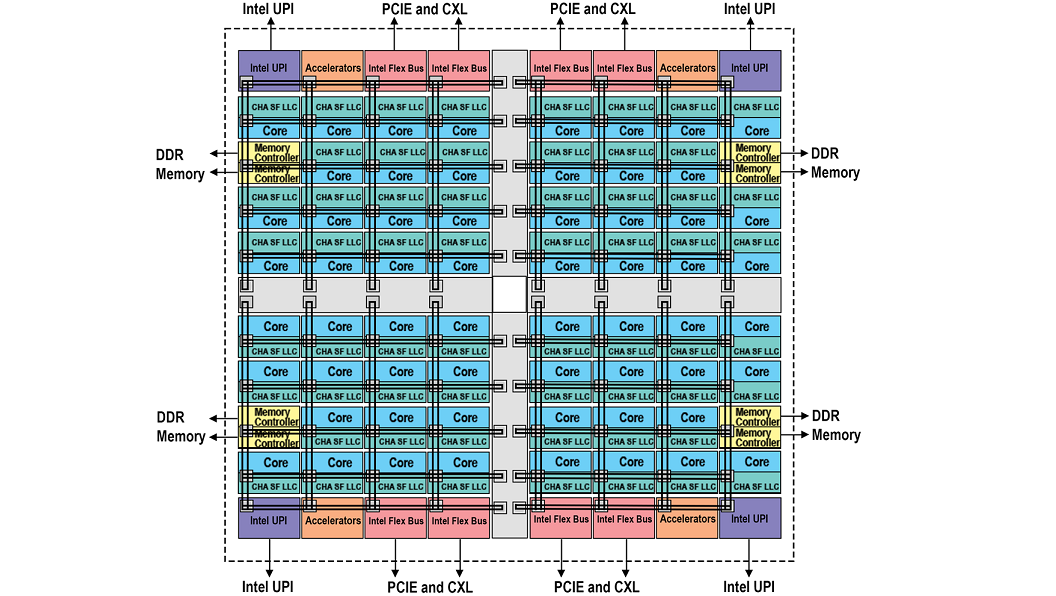
\includegraphics[width=\columnwidth]{fig/spr-uma.png}
    \caption{\label{fig:spr-overview}Block diagram of the 4th Generation Intel Xeon Scalable Processor from~\cite{Intel_4th_gen_scalable}.
Two mirrored tiles are arranged in a 2x2 grid, which are interconnected with EMIB structures to continue the mesh across the die boundaries.~\cite{Intel_2022_ISSCC}}
\end{figure}

\begin{figure}[]
    \begin{subfigure}[t]{0.45\linewidth}
        \centering
        \includegraphics[width=\linewidth]{fig/core-layout/socket0_tikz.pdf}
        \caption{Map of the first socket.}
    \end{subfigure}
    \hfill
    \begin{subfigure}[t]{0.45\linewidth}
        \centering
        \includegraphics[width=\linewidth]{fig/core-layout/socket1_tikz.pdf}
        \caption{Map of the second socket.}
    \end{subfigure}
    \caption{\label{fig:physical-layout}Physical layout of the processor CHA and CPU ids.
	Each box contains two numbers to represent the CHA id followed by a slash and the CPU id, as numbered by the operating system.
	Deactivated CHAs and cores are marked with an X.}
\end{figure}

\section{Test System Details}
I performed all measurements on an Intel Xeon Platinum 8480+ dual socket server.
\tabref{test-system} shows details of the specific test system, called hati.
If not noted otherwise, all measurements on this processor are performed with hyperthreading and SNC-4 activated.
The CPU frequency scaling governor is set to \texttt{performance}.

\begin{table}[t]
	\centering
	\caption{\label{tab:test-system}Test system (hati) details}
	\begin{tabular}{rr}
		\toprule
		Processor	&	2x Intel Xeon Platinum 8480+ (\SI{350}{\watt} TDP)\\
		\rowcolor[HTML]{EFEFEF}Cores		&	2x 56 \\
		Available core frequencies	&	\SI{800}{\MHz} -- \SI{3800}{\MHz} (\SI{2000}{\MHz} nominal) \\
		\rowcolor[HTML]{EFEFEF}Available uncore frequencies	&	\SI{800}{\MHz} -- \SI{2500}{\MHz} \\
		L1-i and L1-d cache	&	112x (\SI{32}{\kibi\byte} + \SI{48}{\kibi\byte})\\
		\rowcolor[HTML]{EFEFEF}L2 cache	&	112x \SI{2048}{\kibi\byte} \\
		L3 cache	&	2x \SI{105}{\mebi\byte} (2d-mesh) \\
		\rowcolor[HTML]{EFEFEF}Mainboard	&	Intel Corporation D50DNP1SB \\
		Memory		&	16x Micron MTC20F2085S1RC48BA1  \\
		 &	\SI{4800}{\mega\hertz} \\
		\rowcolor[HTML]{EFEFEF}Disk		&	Samsung MZQL27T6HBLA-00A07 \\
		OS           &   Ubuntu 22.04 LTS \\
		\rowcolor[HTML]{EFEFEF} Kernel          &   6.8.0 \\
		Power meter & Raritan PX2-5528\\
		\rowcolor[HTML]{EFEFEF} Accuracy & \SI{1}{\percent}\\
		\bottomrule
		%\vspace{6mm}
	\end{tabular}
\end{table}

McCalpin~\cite{McCalpin_2021_CoreMapping} and Cho~\cite{Cho_2022_KnowYourNeighbor} described methods to find the physical location of cores and their associated Caching/Home Agents (CHA).
Schöne created a proof of concept for this measurement on Sapphire Rapids.
It works as follows:
The stream benchmark is executed on each CPU, one after another.
This causes traffic to flow over the mesh the to the DRAM.
First using the vertical interconnect and then the horizontal interconnect~\cite{Intel_2018_SkylakeSP}.
I collect the following performance counters of the mesh traffic from all CHAs:
\begin{itemize}
	\item Vertical Egress Events\footnote{\textbf{TxR\_VERT\_OCCUPANCY0} with AD - Agent 0 and AK - Agent 0: event=144,umask=0x03} to measure the occupancy of the egress buffers in the mesh stop.
	\item Horizontal Egress Events\footnote{\textbf{TxR\_HORZ\_OCCUPANCY} with AD - Uncredited and AK: event=160,umask=0x03} to measure the occupancy of the transgress buffers.
\end{itemize}
This measurement is performed using the default core frequency without the use of hyperthreading.
I use the vertical occupancy event to associate the cores to CHAs.
The horizontal occupancy is used to find which CHAs are in the same row.
I assume that at least one row has not deactived cores and CHAs, and that the ids of the CHAs are numbered sequentially.
This allows me to align the rows and columns to one another around a complete row.
As previously mentioned, sub-NUMA clustering is activated bounding the size of the rows and columns to the size of a tile.
\figref{physical-layout} shows the physical map of the processors core and CHA positions on the test system.

\section{Golden Cove Core Microarchitecture}

Intel published information about the Golden Cove microarchitecture in their optimization reference manual~\cite[Sec. 2.4]{Intel_Optimization_Reference_Manual_050}.
Unlike with previous generations~\cite{Intel_2017_Skylake_SP,Intel_2020_IceLake_SP}, Intel published little information about the internals of their microarchitecture at Hot Chips~\cite{Intel_2021_Hotchips}.
Major tech journalists~\cite{ServerTheHome_2023_SPR_Press,TechGage_2023_SPR_Press,HotHardware_2023_SPR_Press,Wccftech_2023_SPR_Press} have published slides, presumably from the launch event in an coordinated press release on the 10th January 2023.
I was unable to find the original slide deck, thus this information is to be taken with extra caution.

Golden Cove continued to deliver improved instructions throughput compared to previous generations~\cite{Intel_2021_Architecture_Day}.
Kobalicek hosts the asmgrid project~\cite{Kobalicek_AsmGrid} which displays the IPC and latency improvements over the last two generations (Cascade Lake and Ice Lake) and similar products from competitors (Zen 4 and Zen 5).
The likwid bench toolkit~\cite{RHZE_HPC_likwid} would deliver similar results for specific compute kernels.
I was not able to find a publication that describes the IPC improvements based on the data of asmgrid and likwid bench.

Intel increased the size of key structures to enable better out-of-order execution~\cite[Sec. 2.4]{Intel_Optimization_Reference_Manual_050}.
Major changes in the frontend include improved branch prediction, a wider instruction fetch bandwith of \SI{32}{\byte\per cycle}, a 6-way instruction decoder, a bigger μOP Cache and increased bandwith to this cache.
Optimizations for energy efficiency include replacing some operations with microcode.
This causes an increased latency for mixing VEX and SSE instructions if the upper ymm registers are not cleared.~\cite[Sec. 3.11.6]{Intel_Optimization_Reference_Manual_050}
Major changes in the backend include an increased number of allocations, retirement and execution ports.
Especially for execution ports, an additional integer ALU, a second fast floating point adder and one port for AMX instructions was added.
The number of memory access was increased to two \SI{64}{\byte\per cycle} or three \SI{32}{\byte\per cycle} loads and one \SI{64}{\byte\per cycle} or two \SI{32}{\byte\per cycle} stores.~\cite[Sec. 2.4]{Intel_Optimization_Reference_Manual_050}
AMX instructions operate on up to eight tiles each with a maximum size of \SI{1}{\kibi\byte}~\cite[Sec. 20.5.2]{Intel_Optimization_Reference_Manual_050}.

Increasing key structures in the core will inadvertently increase power consumption, this may be offset by the increase in instruction througput for higher energy efficiency.
Since I was only able to find limited amout of public claims from Intel~\cite{Intel_2021_Architecture_Day} about their core microarchitecture, I opted to measure individual components of the core, i.e. reorder buffer, load buffer, store buffer and register file sizes.
Henry Wong created a benchmark that can measure the reorder buffer size~\cite{Wong_2013_robsize} of the out-of-order engine, an essential component that falicitates reordering, idioms and move elimination.
The execution time of two independent pointer chasing loads is measured.
Different filler instructions are inserted between the two loads.
At some number of instructions the latency of the two loads increases, as a limit of some structure in the out-of-order backend is hit.
I implemented the benchmark using C++ and the Asmjit~\cite{Kobalicek_AsmJit} library to generate assembler kernels during runtime.~\footnote{\url{https://github.com/marenz2569/robsize}}
The loop is unrolled \SI{16}{} times and repeated for \SI{2048}{} iterations.
I plot the minimum latency of \SI{16}{} executions of this benchmark with the number of filler instructions between \SI{16}{} and \SI{600}{}.
Each line in the graph is normalized to the minimum and maximum latency over the number of filler instructions.
It is run on CPU 0 with hyperthreading disabled.
To verify the functionality against published values from a primary source~\cite{Intel_2017_Skylake_SP}, the measurement is repeated on the test system (ariel) used Schöne et al. for their benchmarks of Skylake-SP~\cite{Schoene_2019_SKL}.

For measuring the reorder buffer, \textbf{nop} instructions are inserted between the loads.
As~\figref{robsize-reorder} shows, the claim~\cite{ServerTheHome_2023_SPR_Press,Wccftech_2023_SPR_Press} of an out-of-order window with the size \SI{512}{} entries can clearly be validated.
To measure the size of the load and store buffers, I insert \textbf{mov} instructions that load and store from memory to a register.
\figref{robsize-load} shows a discrepancy between the claim~\cite{ServerTheHome_2023_SPR_Press,Wccftech_2023_SPR_Press} of 240 in-flight loads vs the 192 measured.
This has also been measured by Chips and Cheese~\cite{Chipsandcheese_2023_GoldenCove_Vector_Register}, they postulate that Intel is using a different mechanism for in-flight loads.
The difference of 48 entries is equivalent to a size of \SI{3}{\kibi\byte}.
I assume that these are used to support non-temporal loads of AMX tiles which bypass the L1d cache~\cite[Sec. 20.8]{Intel_Optimization_Reference_Manual_050}.
This would allow a minimum of three tiles to reside in a separate load buffer, reducing the negative impact of the large AMX tiles on the out-of-order execution and removing the potential latency of allocating up to 16 entries per tile in the load buffer.
If this is the case, it may be beneficial to have this buffer available to the core if AMX not in use.
In~\figref{robsize-store}, I measure 112 available entries in the store buffer equal to the claim of Intel~\cite{ServerTheHome_2023_SPR_Press,Wccftech_2023_SPR_Press}.
To measure the size of the available number of speculative registers, I insert \textbf{add}, \textbf{mov}, \textbf{cmp} and \textbf{xor} instructions each operating on either the same registers or on two different registers per instruction.
This is repeated for all register types; general purpose (\SI{64}{\bit}), xmm, ymm and zmm registers.
\figref{robsize-registers} shows the measurement of each of the different filler kernels.
I removed zmm registers with \textbf{mov} and \textbf{cmp} filler instructions from the plot as I could not measure latency differences.
Mov elimination, zero ideoms and ones ideoms will cause the jump in measurement latency to appear only after a greater number of filler instructions than the actual size of speculative register files.
Since I cannot measure the register files isolated from the rest of the backend, multiple jumps in latency can be observed for some measurements due to resource limits from different components, i.e. the scheduler.
AVX frequency changes may also influence the measured latencies, as I am running the measurement without setting the core and uncore to a fixed frequency.
Therefore, I use the minimum number of filler instructions that cause a jump as the number of measured speculative registers.
Adding the 32 architectural registers available in the x86-64 ISA gives a lower bound on the number of physical registers.
For Skylake I measure around 148 integer and 132 floating point speculative registers, with 32 registers from the ISA, this leaves no integer and 4 floating point registers unaccounted for~\cite{Intel_2017_Skylake_SP}.
This validates that the measurement can get a close estimate of the number of physical registers.
For Golden Lake I measure 240 integer, 282 xmm/ymm and 188 zmm speculative registers.
This leaves 16 additional integer, 6 xmm/ymm and no zmm physical registers unaccounted for~\cite{ServerTheHome_2023_SPR_Press,Wccftech_2023_SPR_Press}.

The changes of key structures between the Skylake and Golden Cove core architecture are displayed in~\tabref{micro-arch-params}.
\figref{golden-cove} shows a diagram of the Golden Cove core.

\begin{figure}[]
    \centering
    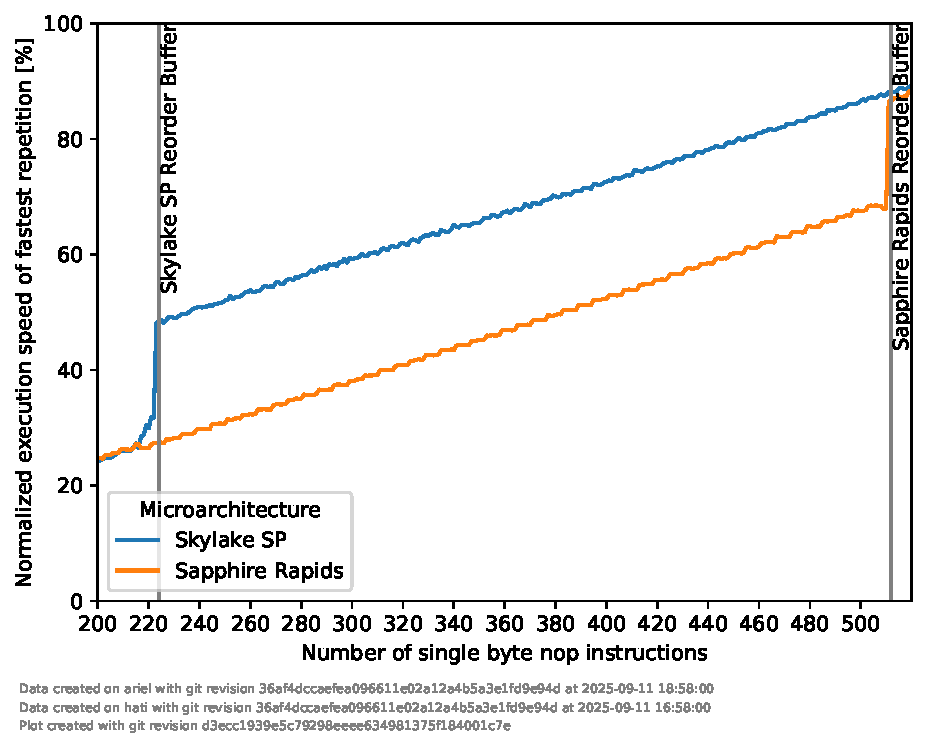
\includegraphics[width=0.8\columnwidth]{fig/robsize/reorder-buffer.pdf}
    \caption{\label{fig:robsize-reorder}Measurement of the reorder buffer size.}
\end{figure}
\begin{figure}[]
    \centering
    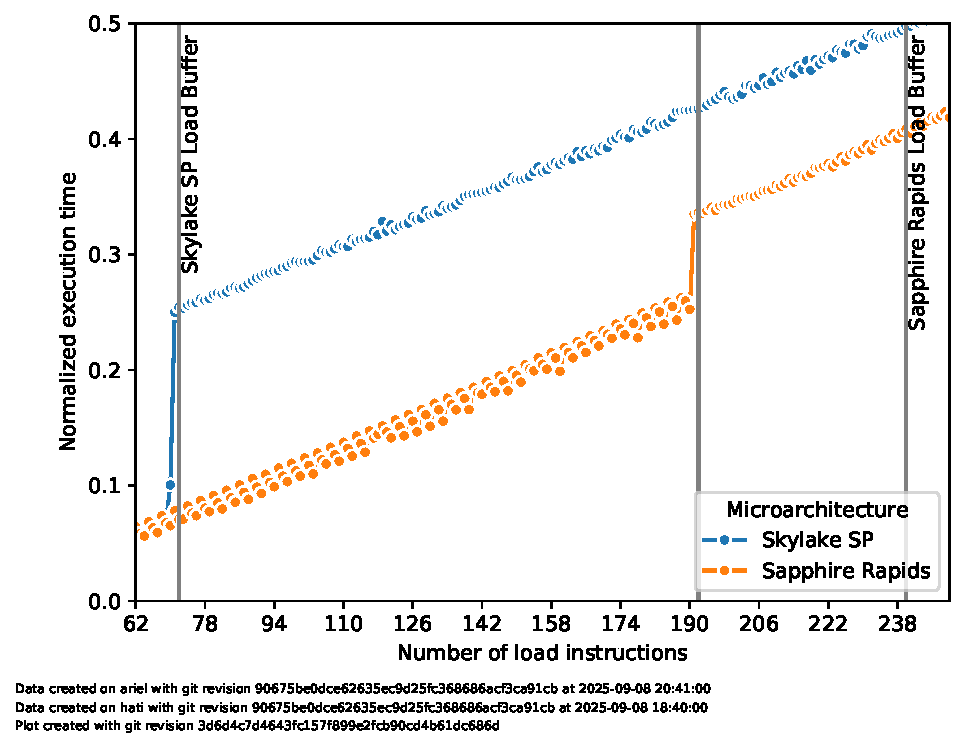
\includegraphics[width=0.8\columnwidth]{fig/robsize/load-buffer.pdf}
    \caption{\label{fig:robsize-load}Measurement of the load buffer size.}
\end{figure}
\begin{figure}[]
    \centering
    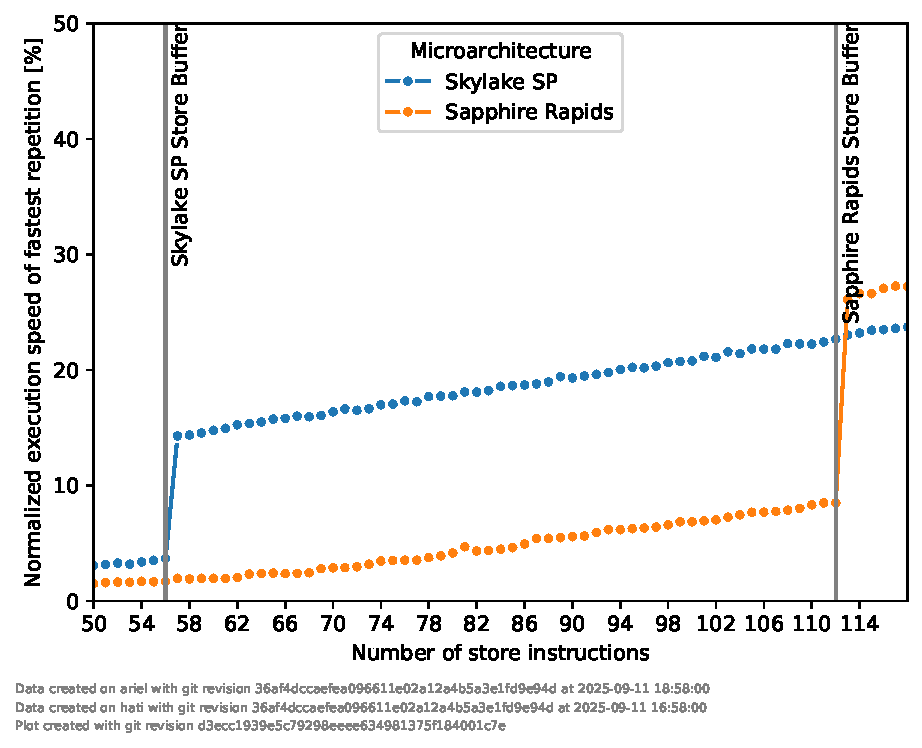
\includegraphics[width=0.8\columnwidth]{fig/robsize/store-buffer.pdf}
    \caption{\label{fig:robsize-store}Measurement of the store buffer size.}
\end{figure}
\begin{figure}[]
    \centering
    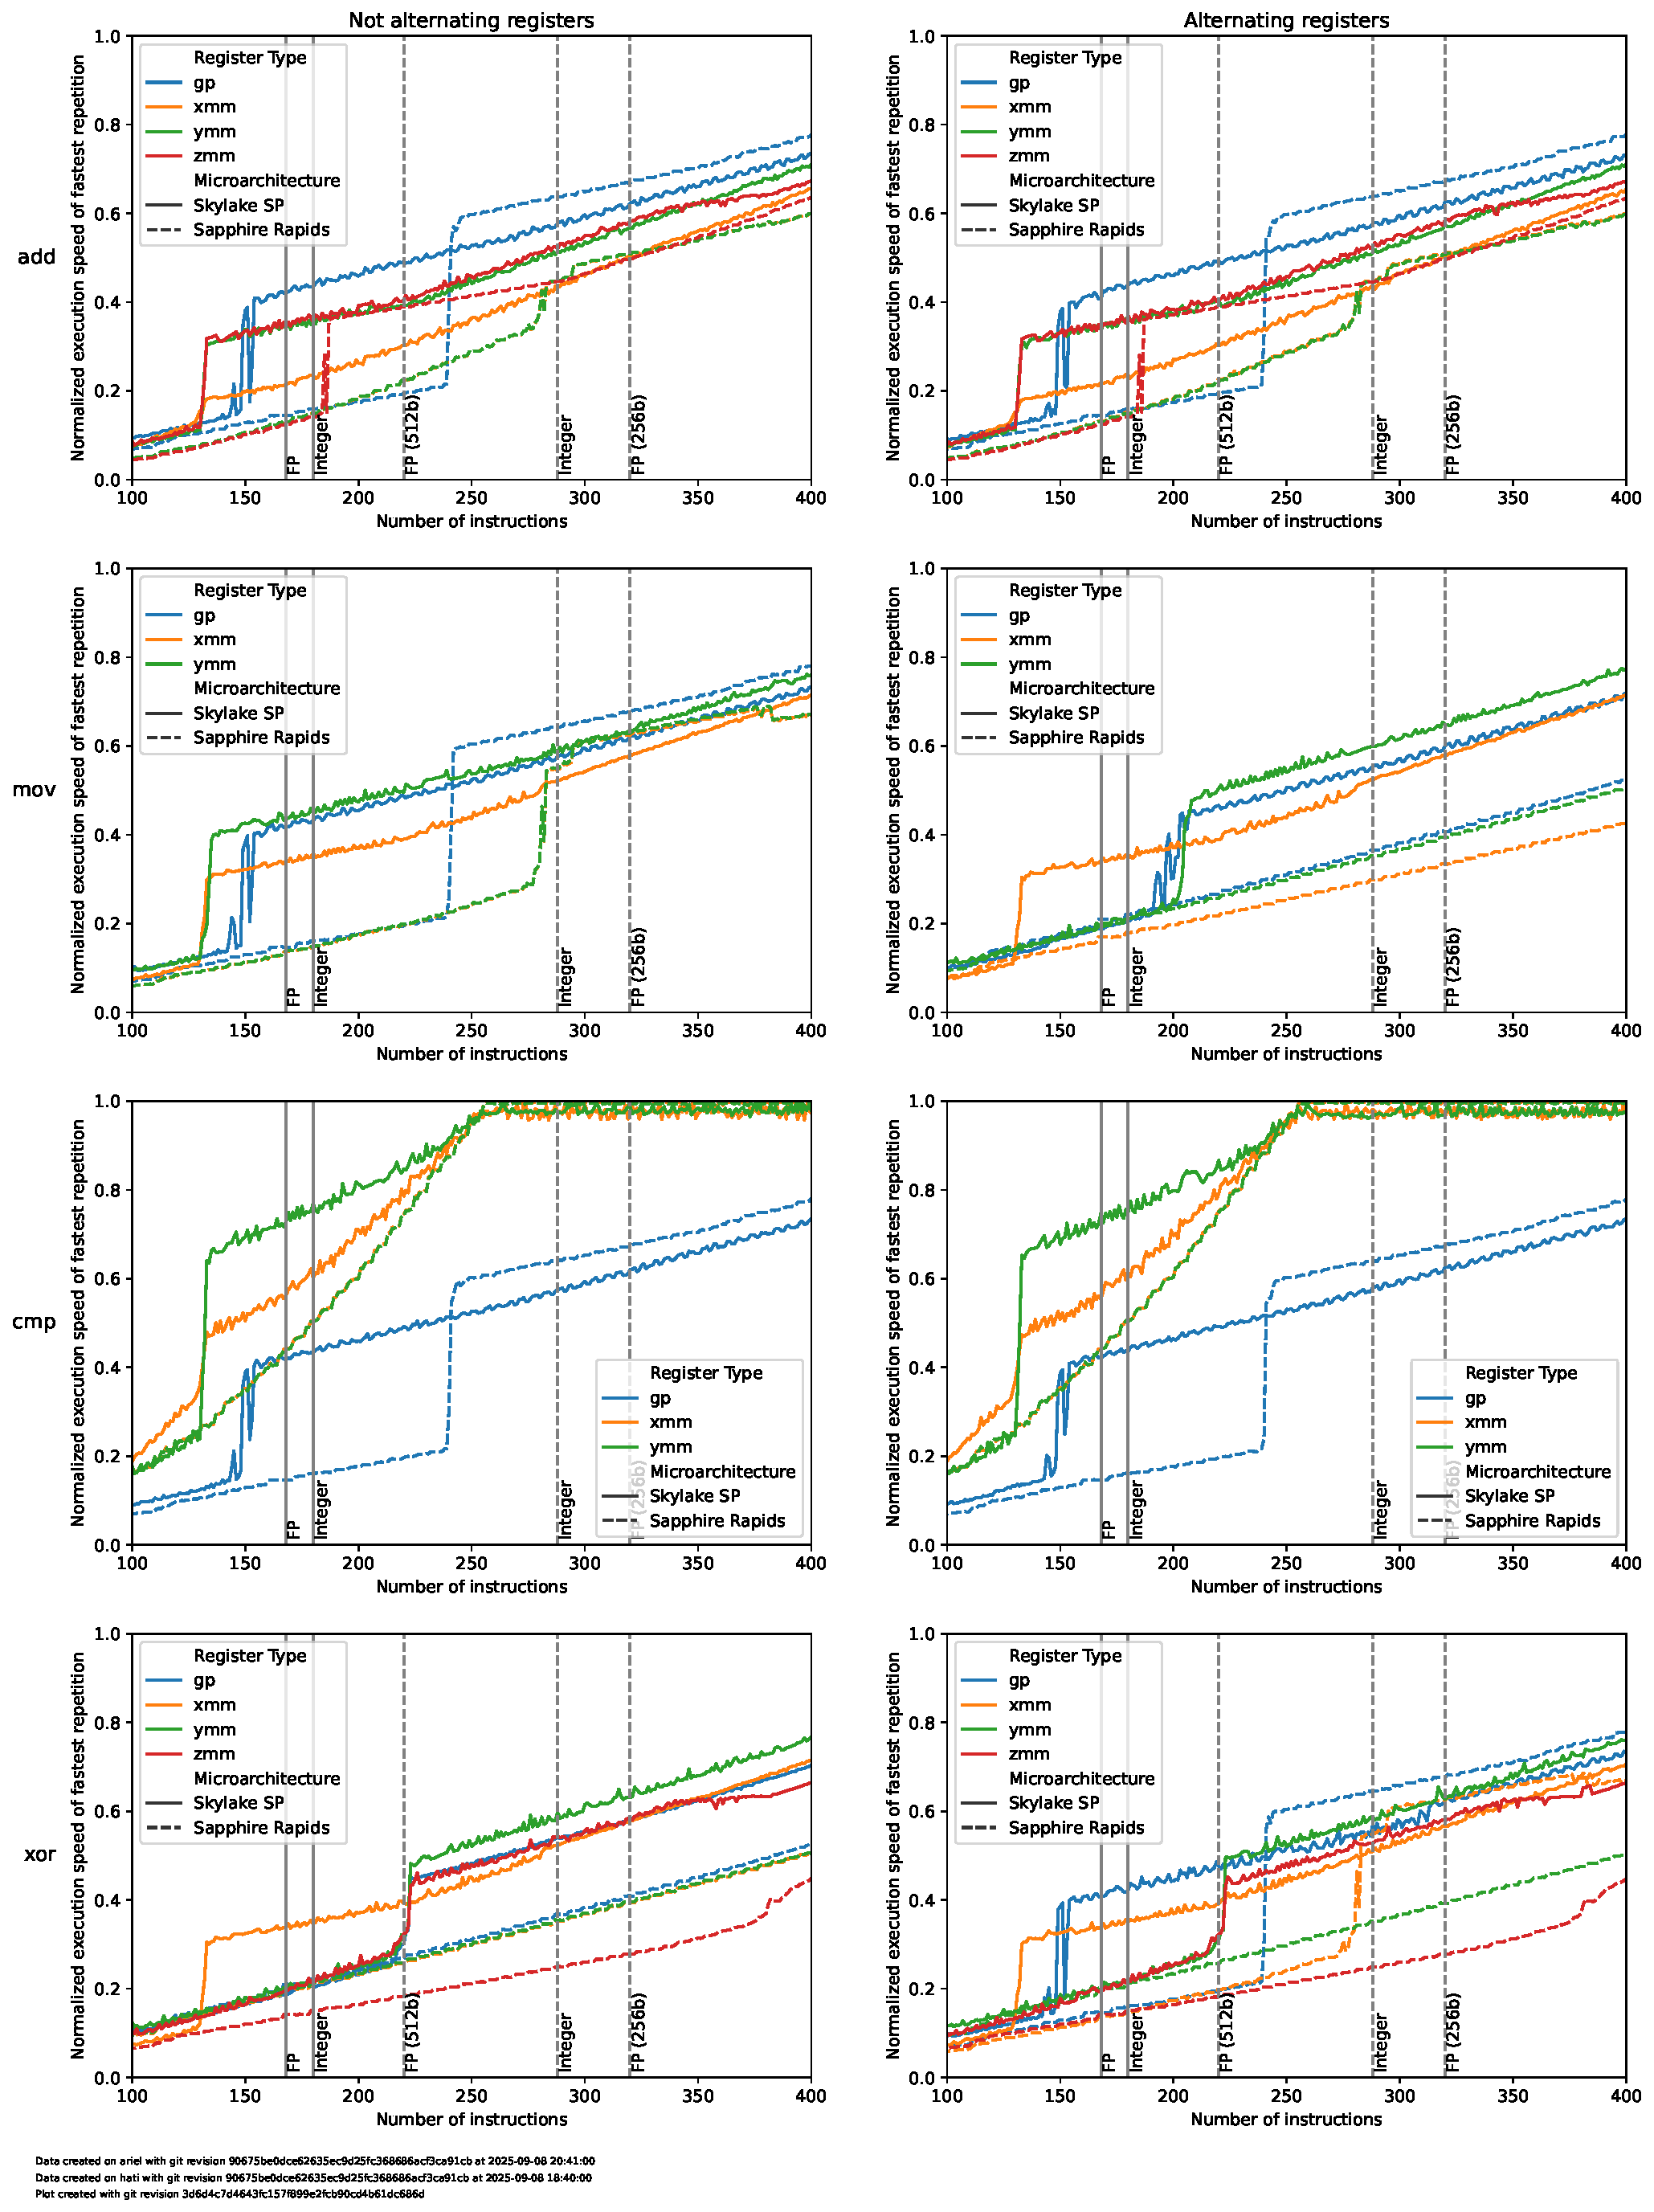
\includegraphics[width=\columnwidth]{fig/robsize/register-files.pdf}
    \caption{\label{fig:robsize-registers}Measurement of the speculative register file sizes based on executing different filler instructions that allocate physical registers.}
\end{figure}

\begin{sidewaystable}[t]
	\centering
	\caption{\label{tab:micro-arch-params}Comparision of key changes between the Skylake and Golden Cove core microarchitecture. Entries that are not from a primary source are either denoted with \checkmark if they have been verified, or ? if they need to be verfied.}
	\begin{tabular}{r|lll}
		\toprule
			&	Skylake & Golden Cove & Golden Cove Verified \\
		\rowcolor[HTML]{EFEFEF}Out-of-order Windows		& 224~\cite{Intel_2017_Skylake_SP} & 512~\cite{Intel_2021_Architecture_Day,ServerTheHome_2023_SPR_Press,Wccftech_2023_SPR_Press} & \checkmark~\figref{robsize-reorder} \\
		In-flight Loads & 72~\cite{Intel_2017_Skylake_SP} & 240~\cite{ServerTheHome_2023_SPR_Press,Wccftech_2023_SPR_Press} & 192 measured in~\figref{robsize-load} \\
		\rowcolor[HTML]{EFEFEF}In-flight Stores & 56~\cite{Intel_2017_Skylake_SP} & 112~\cite{ServerTheHome_2023_SPR_Press,Wccftech_2023_SPR_Press} & \checkmark~\figref{robsize-store} \\
		Register Files Integer & 180~\cite{Intel_2017_Skylake_SP} & 288~\cite{ServerTheHome_2023_SPR_Press,Wccftech_2023_SPR_Press} & $\geq 272$ measured in~\figref{robsize-registers} \\
		\rowcolor[HTML]{EFEFEF}Register Files Floating Point & 168~\cite{Intel_2017_Skylake_SP} & 220 (512b), 320 (256b)~\cite{ServerTheHome_2023_SPR_Press,Wccftech_2023_SPR_Press} & $\geq 220$ (512b), $\geq 314$ (256b) \\
		\rowcolor[HTML]{EFEFEF} & & & measured in~\figref{robsize-registers} \\
		Allocation Queue [\SI{}{\micro OPs\per cycle}]& 64/thread~\cite{Intel_2017_Skylake_SP} & 72/thread, 144 without SMT~\cite{Intel_2021_Architecture_Day,ServerTheHome_2023_SPR_Press,Wccftech_2023_SPR_Press,Intel_Optimization_Reference_Manual_050} & \\
		\rowcolor[HTML]{EFEFEF}μOP Cache [\SI{}{\micro OPs\per core}] & \SI{1536}{}~\cite{Wikichip_SkylakeSP} & \SI{4096}{}~\cite{Intel_2021_Architecture_Day} & ? measurement proposed \\
		\rowcolor[HTML]{EFEFEF} & & & in~\cite{Schoene_2021_FIRESTARTER2} \\
		Number of decoder & \SI{4}{}~\cite{Wikichip_SkylakeSP} & \SI{6}{}~\cite{Intel_2021_Architecture_Day,Intel_Optimization_Reference_Manual_050} & \\
		\rowcolor[HTML]{EFEFEF}L1i Cache Bandwidth [\SI{}{\byte\per cycle}] & \SI{16}{}~\cite{Wikichip_SkylakeSP} & \SI{32}{}~\cite{Intel_Optimization_Reference_Manual_050} & \\
		L1i TLB & 4K: 64 & 4K: 256 & \checkmark verified via \textbf{cpuid} \\
		  & 2M+4M: 8~\cite{Wikichip_SkylakeSP} & 2M+4M: 32~\cite{Intel_2021_Architecture_Day,Intel_Optimization_Reference_Manual_050} & \\
		\rowcolor[HTML]{EFEFEF}L1d Load Bandwidth [\SI{}{\byte\per cycle}] & 2x\SI{64}{}~\cite{Intel_2017_Skylake_SP} & 3x\SI{32}{} or 2x\SI{64}{}~\cite{Intel_Optimization_Reference_Manual_050} & \\
		L1d Store Bandwidth [\SI{}{\byte\per cycle}] & 1x\SI{64}{}~\cite{Intel_2017_Skylake_SP} & 2x\SI{32}{} or 1x\SI{64}{}~\cite{Intel_Optimization_Reference_Manual_050} & \\
		\rowcolor[HTML]{EFEFEF}L1d TLB & 4K: 64                          & all page sizes: 8 (store only) & \checkmark verified via \textbf{cpuid} \\
		\rowcolor[HTML]{EFEFEF}        & 2M+4M: 32                       & 4K: 64 (load only)  & \\
		\rowcolor[HTML]{EFEFEF}        & 1G: 4~\cite{Wikichip_SkylakeSP} & 2M+4M: 32 (load only)  & \\
		\rowcolor[HTML]{EFEFEF}        &                                 & 1G: 8 (load only) & \\
		L1d Line Fill Buffer & \SI{10}{entries}~\cite{Wikichip_SkylakeSP} & \SI{16}{entries}~\cite{Intel_2021_Architecture_Day} & ? \\
		\rowcolor[HTML]{EFEFEF}L2 Unified TLB & 4K+2/4M: 1536 & 4K: 2048 & \checkmark verified via \textbf{cpuid} \\
		\rowcolor[HTML]{EFEFEF}  & 1G: 16~\cite{Intel_2017_Skylake_SP} & 2+4M and 1G: 1024 each shared with 4K~\cite{ServerTheHome_2023_SPR_Press,Wccftech_2023_SPR_Press} & \\
		\bottomrule
		%\vspace{6mm}
	\end{tabular}
\end{sidewaystable}


\begin{figure}[]
    \centering
    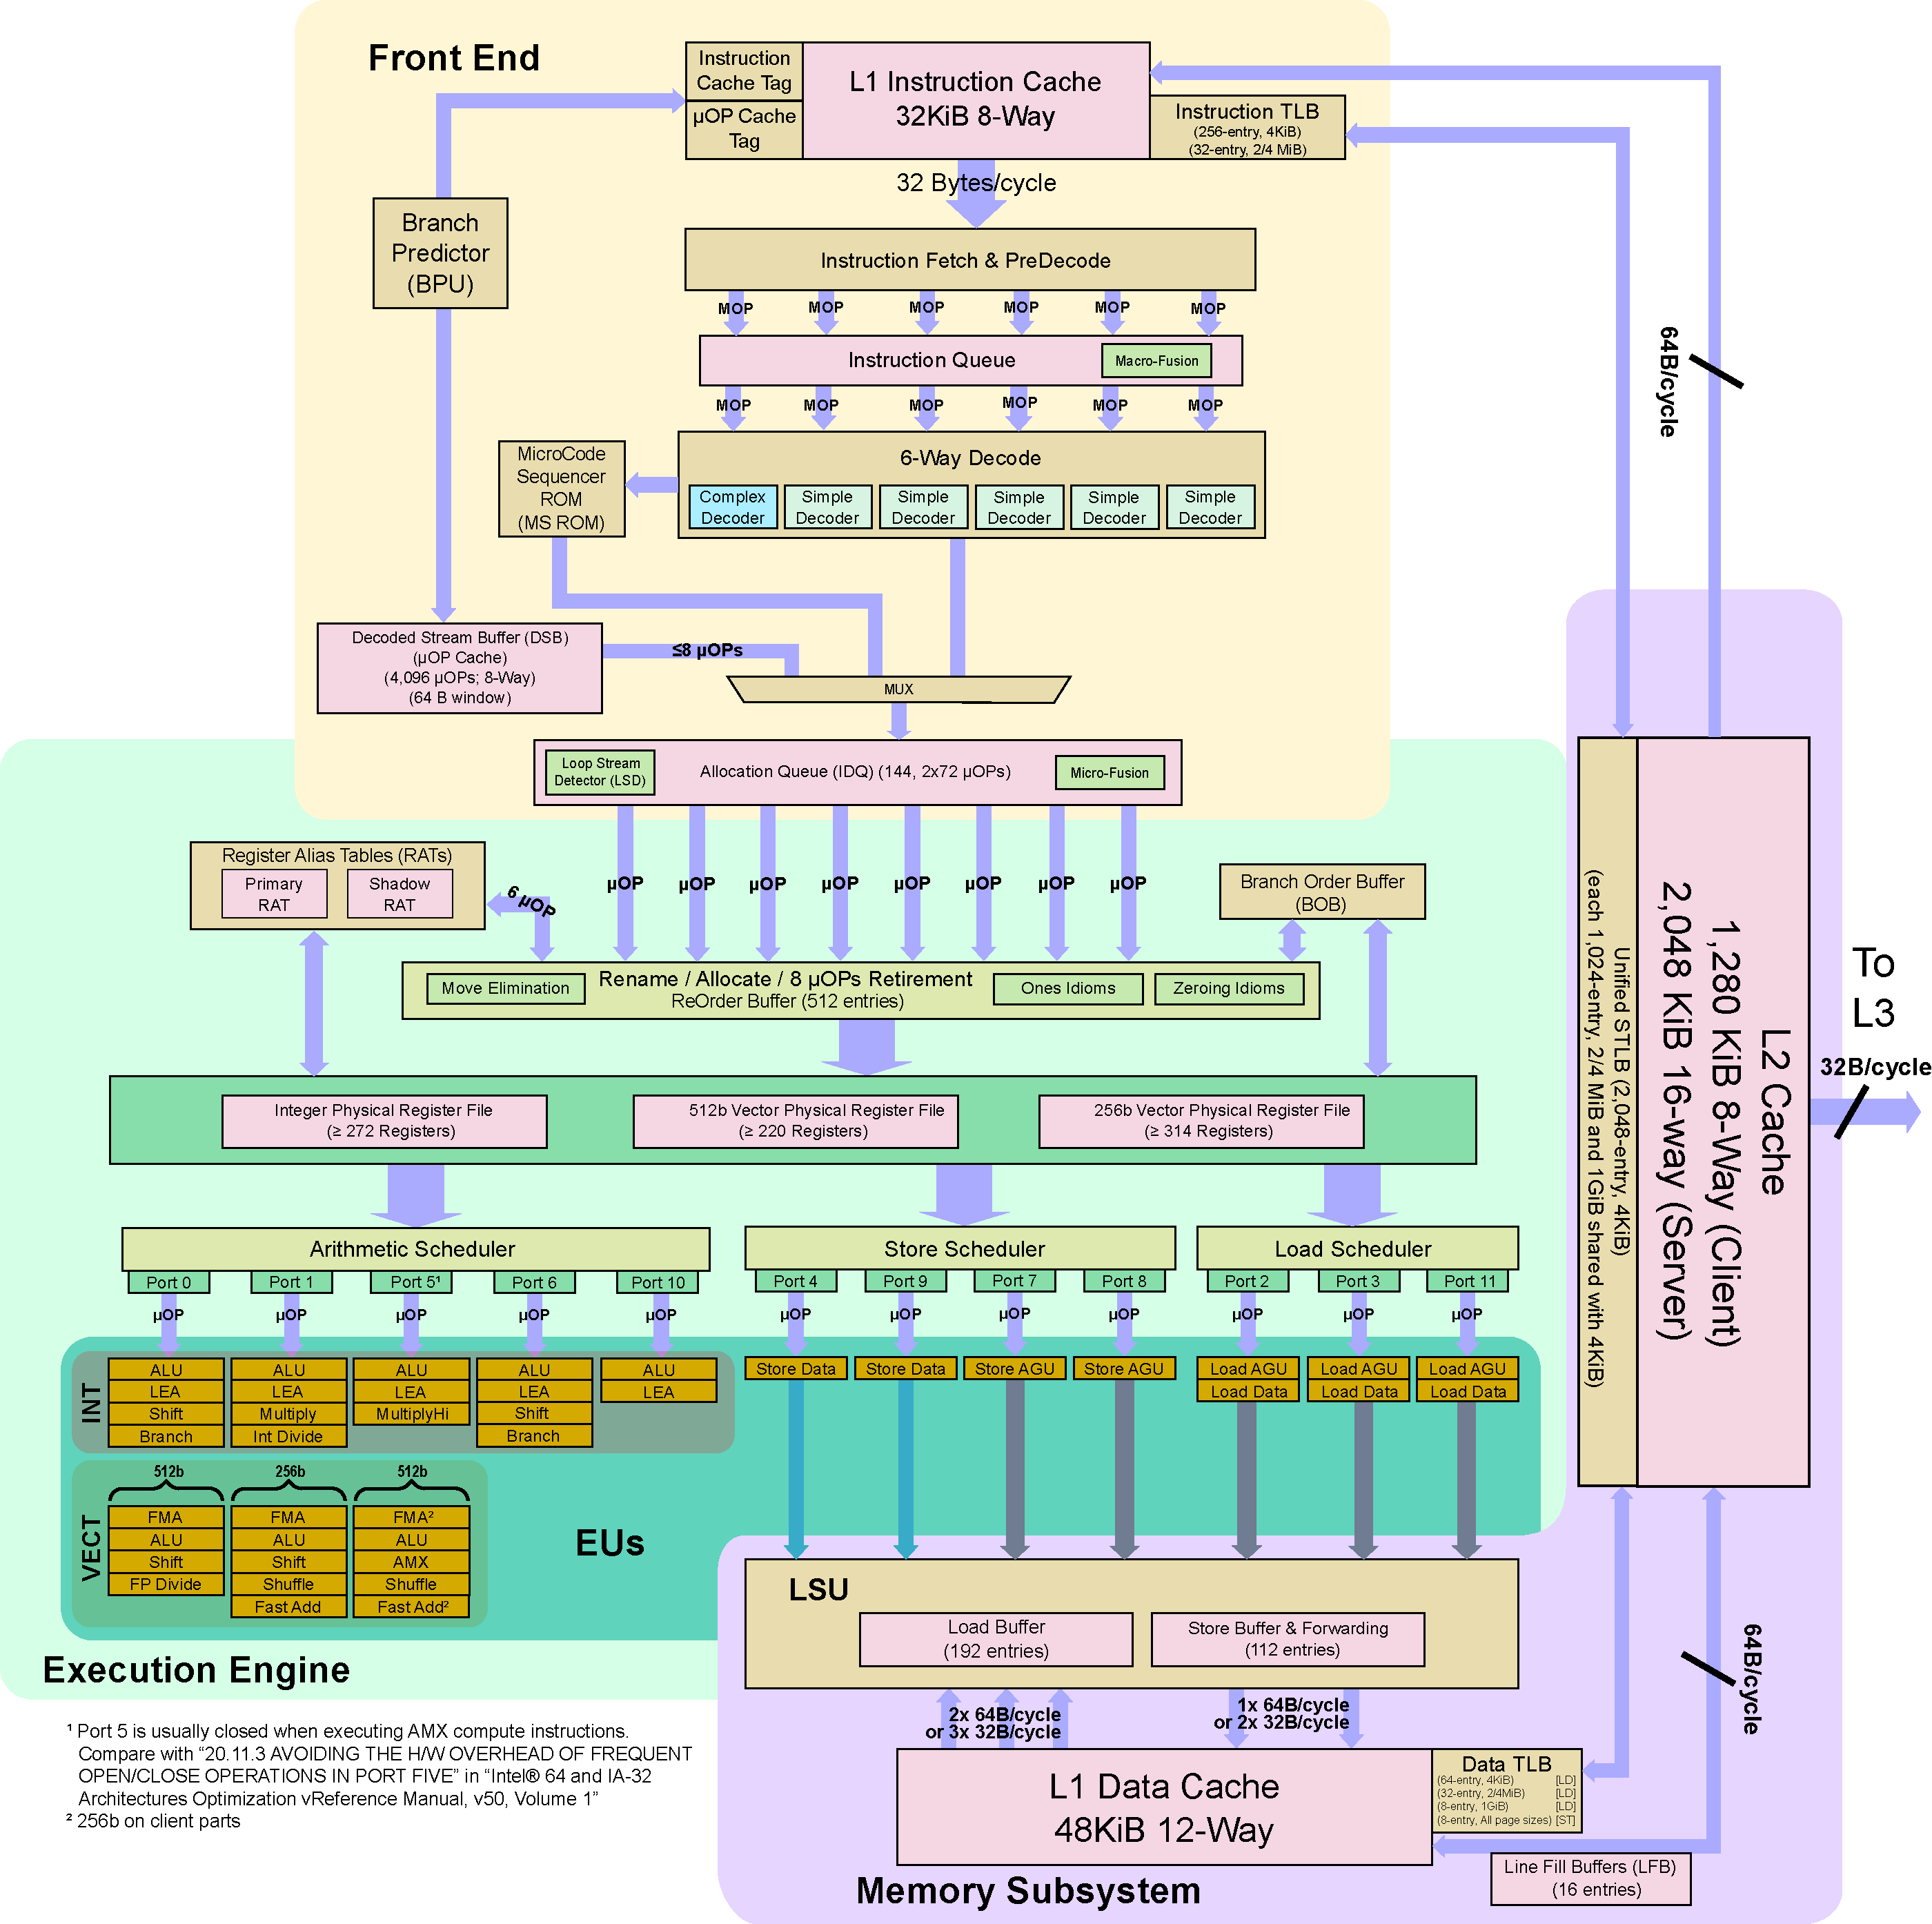
\includegraphics[width=\columnwidth]{fig/GoldenCoveCore.pdf}
    \caption{\label{fig:golden-cove}Block diagram of the Golden Cove Core, based on the Figure published by WikiChip~\cite{Wikichip_SunnyCoveDiagram} for the predecessor Sunny Cove.}
\end{figure}

\clearpage

\section{L3 Cache Slicing}
\label{sec:l3_cache_slicing}

The 2d-mesh design of Intels L3 caches poses a unique opportunity for optimizing communication latency between two cores.
McCalpin demonstrated that each cache line is associated to a L3 cache slice based on a hash algorithm, which differs for each SKU~\cite{McCalpin_2018_IntelAddressHashing}.
Therefore communication latency of two cores using a specific cache line depends on the physical locations of the cores and the cache slice associated to this particular cache line.

I run a benchmark that sends \SI{100}{} ping/pong signals on a cache line shared by two cores using the atomic \textbf{lock cmpxchg} instruction.
The latency of the ping/pongs is measured using the timestamp counter.
To account for cache slicing, I repeat the measurement \SI{100}{} times on \SI{1000}{} different cache lines.
Memory is allocated in the sub-NUMA cluster of the ping core.
The latency of one cache line is modeled using a normal distribution over all repetitions.
Kmeans clustering is used to create \SI{14}{} clusters (equivalent to the number of cache boxes in on sub-NUMA cluster) using the mean latency of the modeled cache lines.
Hyperthreading is disabled and the measurement is repeated on the cross product of following settings:
\begin{itemize}
    \item Each 2-tuple of different cores on the first socket
    \item Core frequency set to \SI{800}{\MHz}, \SI{2000}{\MHz} and \SI{3800}{\MHz} (turbo)
    \item Uncore frequency set to \SI{800}{\MHz} and \SI{2500}{\MHz}
\end{itemize}

\figref{cbo-latencies} shows the distinct communication latencies between two cores in the same sub-NUMA cluster using the \SI{14}{} cache boxes.
A slight mismatch between the distribution of cache lines across different cache slices is visible.
This effect is described by McCalpin~\cite{McCalpin_2018_IntelAddressHashing} as an artifact of using specific hash algorithms.

\begin{figure}[]
    \centering
    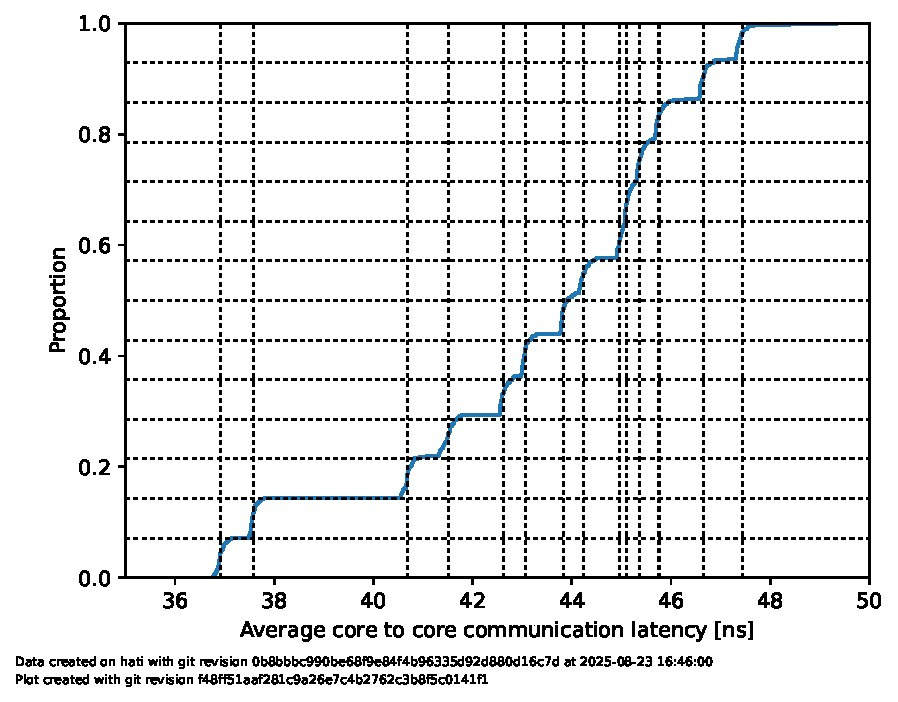
\includegraphics[width=0.8\columnwidth]{fig/core-to-core-latency/core0to1latency.pdf}
    \caption{\label{fig:cbo-latencies}Cumulative distribution of the communication latencies between cores 0 and 1 running with \SI{3800}{\MHz} core and \SI{2500}{\MHz} uncore frequency.
    Vertical lines show the centroids of the kmeans clustering.
    Horizontal lines are equally spaced.}
\end{figure}

\begin{figure}[]
    \centering
    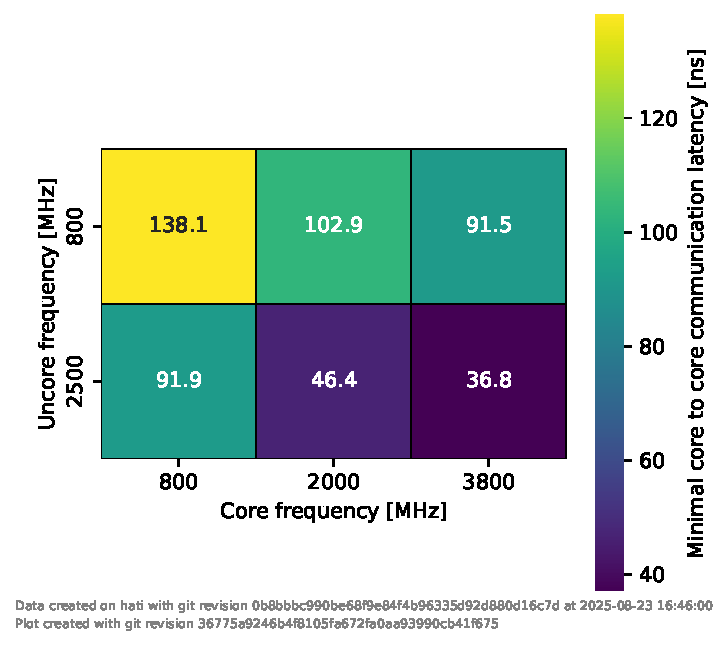
\includegraphics[width=0.8\columnwidth]{fig/core-to-core-latency/all-to-all-heatmap-min.pdf}
    \caption{\label{fig:cbo-latencies-socket-min}Minimal core to core communication latency over all cores of hati's socket 0.}
\end{figure}
% \begin{figure}[]
%     \centering
%     \includegraphics[width=0.8\columnwidth]{fig/core-to-core-latency/all-to-all-heatmap-mean.pdf}
%     \caption{\label{fig:cbo-latencies-socket-mean}Average core to core communication latency over all cores of hati's socket 0.}
% \end{figure}
\begin{figure}[]
    \centering
    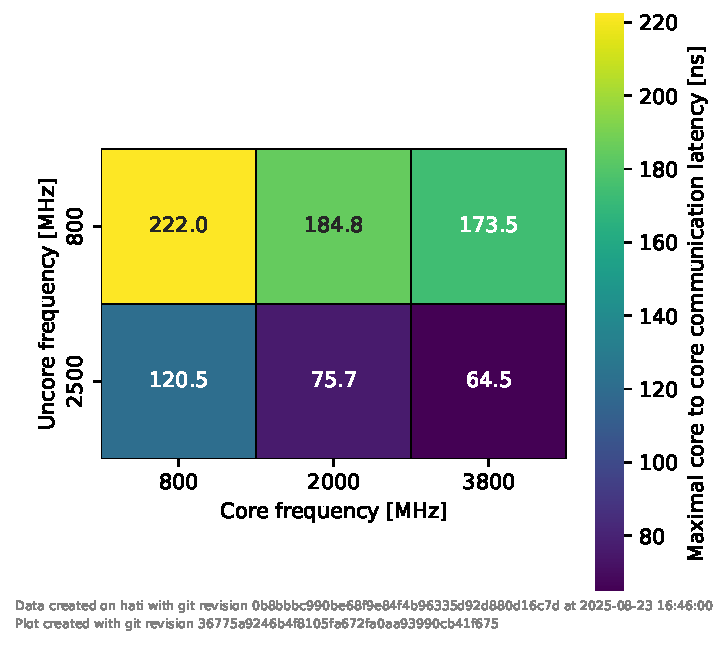
\includegraphics[width=0.8\columnwidth]{fig/core-to-core-latency/all-to-all-heatmap-max.pdf}
    \caption{\label{fig:cbo-latencies-socket-max}Maximal core to core communication latency over all cores of hati's socket 0.}
\end{figure}
\begin{figure}[]
    \centering
    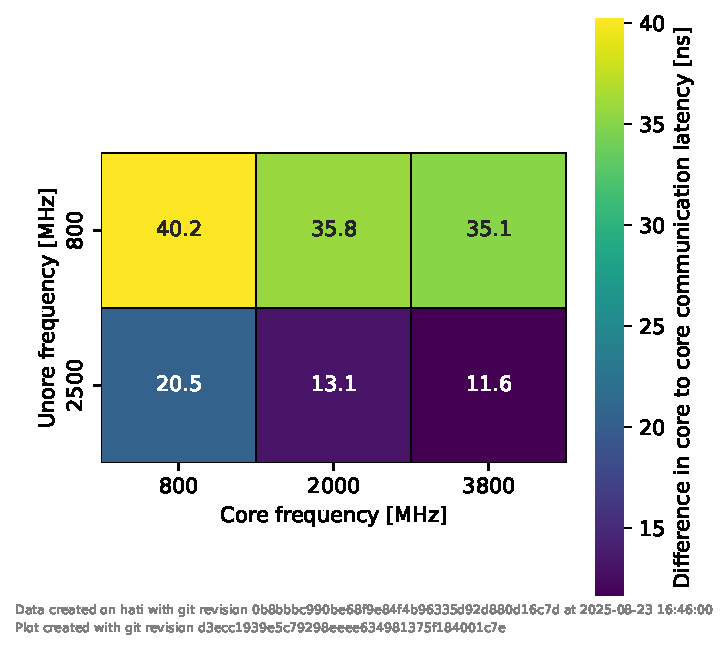
\includegraphics[width=0.8\columnwidth]{fig/core-to-core-latency/all-to-all-heatmap-diff.pdf}
    \caption{\label{fig:cbo-latencies-socket-diff}Difference in core to core communication latency over all cores of hati's socket 0.}
\end{figure}

The measurement enables building a model showing how the different core and uncore frequencies influence communication latencies.
\figref{cbo-latencies-socket-min}, \figref{cbo-latencies-socket-max} and \figref{cbo-latencies-socket-diff} show the minimum, maximum and maximal difference in communication latencies over all pairs of cores on the first socket.
% \figref{cbo-latencies-socket-min}, \figref{cbo-latencies-socket-mean}, \figref{cbo-latencies-socket-max} and \figref{cbo-latencies-socket-diff} show the minimum, average, maximum and difference in communication latencies over all pairs of cores on the first socket.
The plots for the latencies of specific core combinations are included in~\appref{core_to_core_latencies_complete}.

I create a model of core to core latency using linear regression with the core and uncore frequency as parameters:
\begin{equation*}
t_{latency}~[ns] = a + \frac{b}{f_{core}~[MHz]} + \frac{c}{f_{uncore}~[MHz]}
\end{equation*}
The computed parameters are displayed in~\tabref{latency_model_parameters}.
Each of the models have a coefficient of determination $R^2 > 0.99$, leaving little variability unaccounted for.
The latency plots for all core and uncore frequency combinations using this model are included in~\appref{core_to_core_latencies_model}.

The presented methodology shows that latencies of core to core communication can be easily modeled.
It can be extended to show latencies inside a single NUMA node or across sockets utilizing the UPI link.
Note that the models should be considered best case scenarios, as the 2d-mesh interconnect is not congested by traffic, which would increase the observed latencies.

\begin{table}[t]
	\centering
	\caption{\label{tab:latency_model_parameters}Parameters of the latency models}
	\begin{tabular}{rrrr}
		 & Parameter $a$ & Parameter $b$ & Parameter $c$ \\
		\toprule
		\rowcolor[HTML]{EFEFEF}Minimal latency & $-1.2283117081191506$ & $52020.30476702$ & $61732.83781473$ \\
		Maximal latency & $0.9258637728757435$ & $53374.66379634$ & $125374.30302008$ \\
		\rowcolor[HTML]{EFEFEF}Maximal difference in latency & $-0.1620055737606272$ & $7294.88075747$ & $25821.70896832$ \\
		\bottomrule
		%\vspace{6mm}
	\end{tabular}
\end{table}


Performance engineers optimizing for the last percent require intricate knowledge about the core and uncore microarchitecture.
This should ideally be facilitated by continuous tracking and automated benchmarking across generations.
Latency critial applications can optimize communication by using specific core and memory pinnings.
Selecting the cache lines used for communication can reduce latency in an order of \SI{17}{\percent}.